\documentclass[12pt,a4paper]{paper}
\usepackage[brazil]{babel}
\usepackage[T1]{fontenc}
\usepackage[utf8]{inputenc}
\usepackage[letterpaper,top=2cm,bottom=2cm,left=2cm,right=2cm,marginparwidth=1.75cm]{geometry}

\usepackage{amsmath}
\usepackage{graphicx}
\usepackage{cite}
\usepackage{xurl}
\usepackage[hidelinks]{hyperref}
\usepackage[printonlyused]{acronym}
\usepackage{microtype}

\usepackage{booktabs}
\usepackage{tabularx}
\usepackage{array}

\newcolumntype{L}[1]{>{\raggedright\arraybackslash}p{#1}}
\newcolumntype{Y}{>{\raggedright\arraybackslash}X}

\usepackage{multirow}
\usepackage{longtable}

\usepackage{indentfirst}
\setlength{\parindent}{0.5cm}

\usepackage{tikz}
\usetikzlibrary{arrows.meta, positioning, calc}

\usepackage{siunitx}

\usepackage{import}

\title{IoT na Agricultura: Colheita Autônoma com Robôss Voadores da Tevel}
\author{Matheus Renó Torres}
\date{}

\begin{document}
\maketitle

% \begin{abstract}

% \end{abstract}

%\textbf{Palavras-chave:} 

\acrodef{IoT}{Internet of Things}
\acrodef{VANT}{Veículo Aéreo Não Tripulado}
\acrodefplural{VANT}{Veículos Aéreos Não Tripulados}
\acrodef{FAR}{Flying Autonomous Robot}
\acrodef{GPU}{Graphics Processing Unit}
\acrodef{MQTT}{Message Queuing Telemetry Transport}

\section{Introdução}

A Tevel Aerobotics Technologies desenvolveu os \ac{FAR}, \acp{VANT} para colheita seletiva de frutas, com aplicações divulgadas em pomares na Itália, EUA e Chile~\cite{tevel2026}. Este estudo analisa o produto como sistema de robótica, \ac{IoT} e computação de borda~\cite{reeuwijk2025}, com foco na colheita de maçãs. A operação relatada pela Unifrutti em Linares, Chile, é a principal evidência de implementação analisada~\cite{unifrutti2023tevel}.
\section{Problema e Objetivo}

O problema é a escassez de mão de obra na colheita. A Tevel associa essa restrição à dificuldade de colher no momento adequado e propõe a automação para reduzir a dependência de trabalhadores sazonais~\cite{tevel2026,unifrutti2023tevel}. O desafio é adequar a capacidade de coleta à janela de maturação: atrasos comprometem o objetivo agronômico, enquanto a colheita indiscriminada elimina a seletividade.

Neste estudo, a quantidade de frutos comercializáveis colhidos com qualidade constitui o critério de desempenho operacional. Movimentos executados ou frutos detectados, isoladamente, não representam a efetividade da colheita. Segundo a Unifrutti, a operação em seus pomares realizou colheita seletiva, depositou os frutos em recipientes e minimizou contusões. O comunicado também descreve o acesso à quantidade colhida e a dados de peso, classificação por cor, maturação, diâmetro, horário e geolocalização dos frutos, permitindo caracterizar a produção e sua qualidade~\cite{unifrutti2023tevel}.
\section{Produto e Arquitetura Física}

O produto combina robôs aéreos e uma estação terrestre móvel. Segundo relato técnico da Spectro Cloud de 2025, a estação concentra \acp{GPU} de alto desempenho, e cada robô utiliza ventosas para coleta e um cabo para energia e dados~\cite{reeuwijk2025}. Essa organização mantém o processamento intensivo no solo, reduzindo o hardware computacional transportado em voo.

\begin{figure}[!htb]
    \centering
    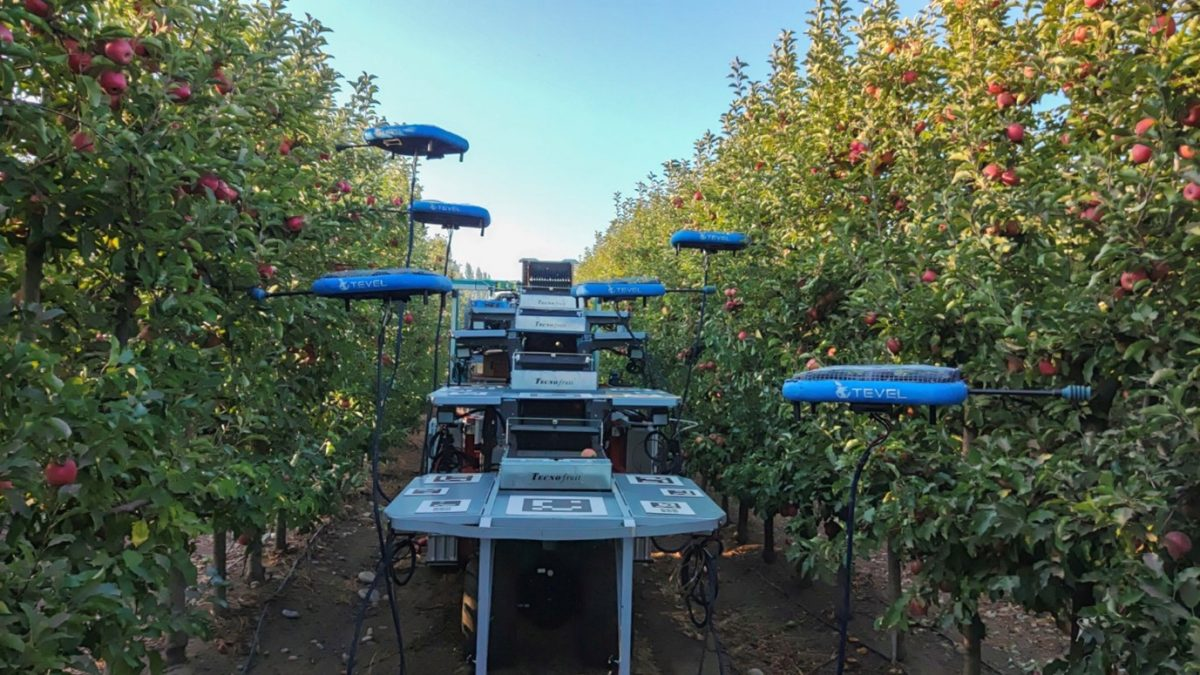
\includegraphics[width=0.98\linewidth]{figures/tevel_unufrutti.png}
    \caption{Robôs da Tevel em operação nos pomares da Unifrutti em Linares, Chile~\cite{unifrutti2023tevel}.}
    \label{fig:tevel_unifrutti}
\end{figure}

Na implantação chilena, oito \acp{FAR} foram integrados à plataforma de colheita da Darwin Harvesting Group, que recebia os frutos em recipientes~\cite{unifrutti2023tevel}. Essa quantidade caracteriza a implementação relatada, sem estabelecer uma configuração obrigatória para todas as versões.

A Tevel descreve detecção de frutos, folhagem e outros objetos, classificação por tamanho e maturação, rastreamento de frutos, fusão de dados, planejamento e execução de trajetórias e estabilização sob forças da folhagem e dos frutos~\cite{tevelTechnology}. Funcionalmente, a missão encadeia percepção, seleção do alvo, aproximação, desprendimento e entrega. A identificação correta do alvo não assegura acesso ou desprendimento adequados.

A publicação de patente WO2018033922A1 descreve navegação em malha fechada para aproximação e interação com frutos, mecanismos de coleta e estruturas de proteção entre folhas e galhos~\cite{maor2018harvesting}. Essas alternativas esclarecem a abordagem de engenharia, mas não comprovam a composição do produto comercial nem substituem os registros de operação que demonstram sua aplicação.

Como interpretação arquitetural, a autonomia resulta do conjunto aéreo-terrestre. A concentração de recursos no solo favorece o compartilhamento computacional e condiciona o desempenho à estação e aos enlaces locais. O compartilhamento de recursos e as restrições de movimento impostas pelos cabos devem ser considerados na adaptação ao pomar.
\section{Arquitetura IoT, Comunicação e Dados}

A Figura~\ref{fig:sintese_arquitetura} sintetiza os enlaces entre os \ac{FAR} e a plataforma terrestre, a interface do operador e a gestão remota da infraestrutura~\cite{reeuwijk2025,oliveira2023tevel}.

\begin{figure}[!htb]
    \centering
    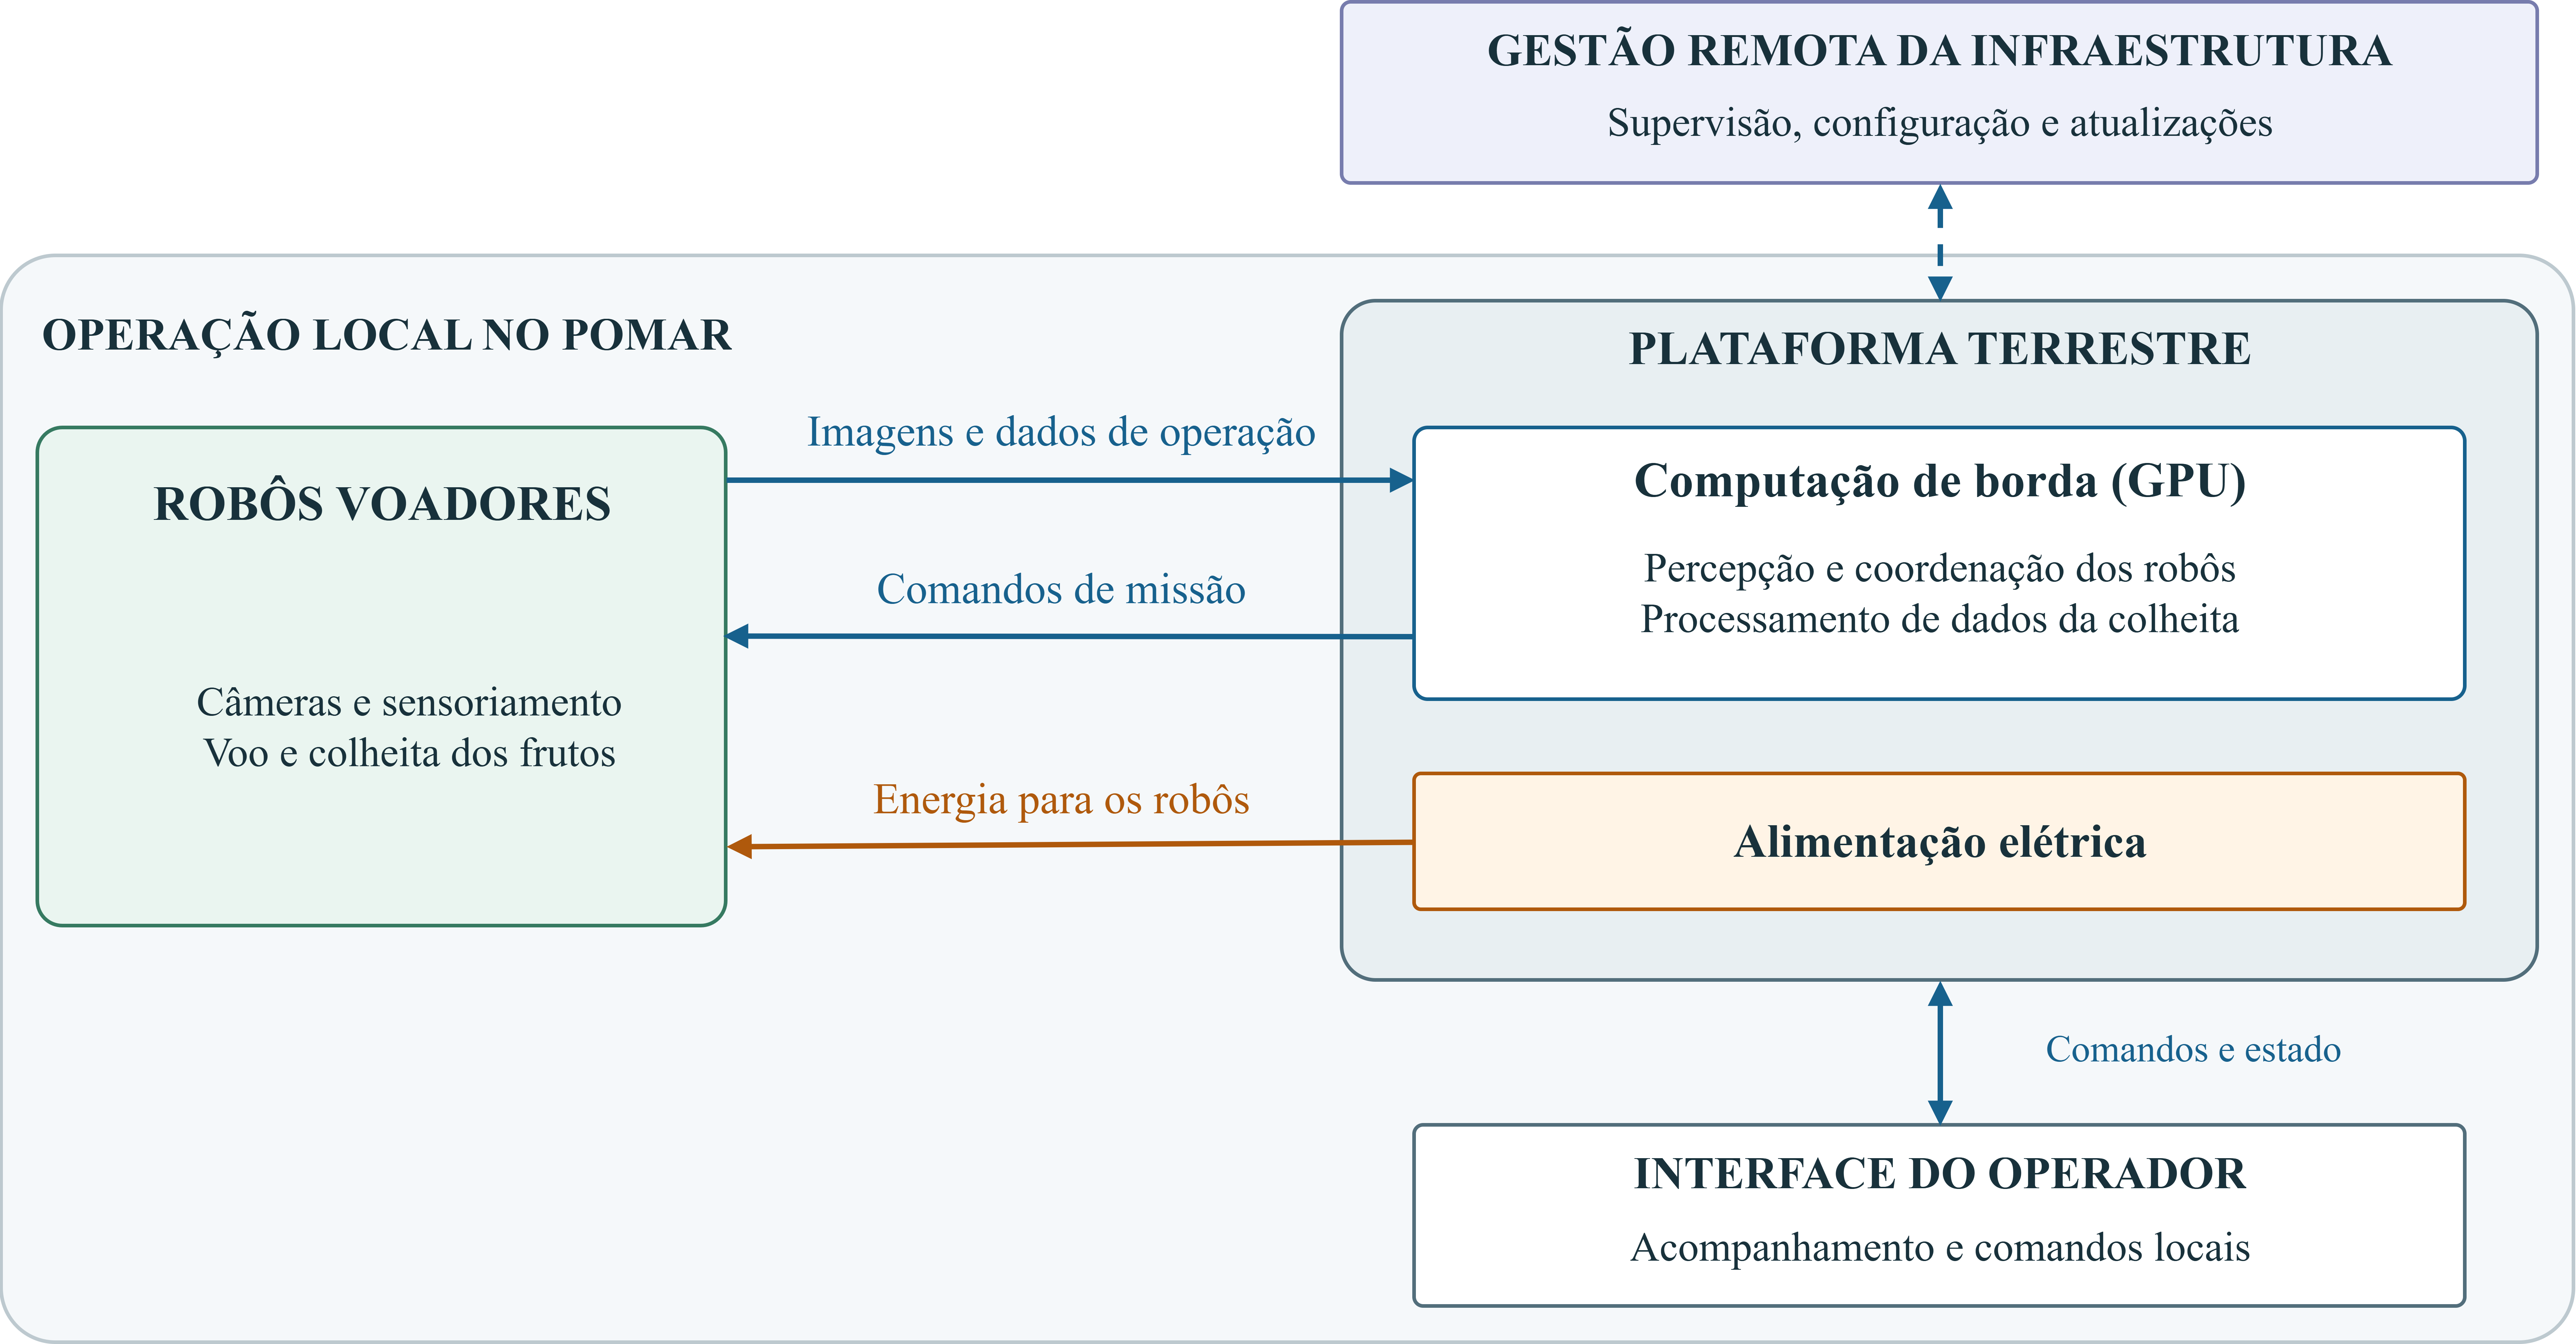
\includegraphics[width=0.98\linewidth]{figures/arquitetura_tevel.drawio.png}
    \caption{Síntese funcional da arquitetura.}
    \label{fig:sintese_arquitetura}
\end{figure}

Na apresentação de 2023, Tevel e Spectro Cloud destacam conectividade instável, dificuldade de acesso às instalações e operação durante desconexões. O material distingue a gestão remota dos ambientes de borda e apresenta a operação desconectada como requisito~\cite{oliveira2023tevel}. Essa organização visa manter as aplicações locais em execução quando a gestão remota estiver indisponível.

Esse requisito não demonstra tolerância à ruptura do cabo, à perda de alimentação ou à falha do computador terrestre, cujas respostas não são especificadas nas fontes consultadas. Tampouco se apresenta uma descrição completa dos protocolos entre robôs, estação e infraestrutura externa. Sem confirmação documental, não se atribuem ao produto \ac{MQTT}, LoRaWAN, 5G ou Ethernet.

A Tevel declara disponibilizar quantidade colhida, peso e tamanho dos frutos, classificação por cor, detecção de doenças, horário, geolocalização e distribuições de peso, tamanho e cor por recipiente~\cite{tevelTechnology}. Esses registros associam os frutos à sua representação digital e informam ao produtor a composição da colheita antes do beneficiamento.

A utilidade dos dados depende de rastreabilidade e qualidade. Sua avaliação exige distinguir medições de estimativas por visão, registrar falhas de aquisição e verificar a exatidão das classificações. As fontes consultadas não detalham todos os sensores, a calibração, a incerteza do peso ou a acurácia da detecção de doenças. A funcionalidade anunciada, portanto, não comprova desempenho metrológico ou diagnóstico validado.
\section{Computação}

A documentação pública identifica componentes de software, mas não detalha toda a eletrônica. A apresentação conjunta de 2023 descreve a evolução de instalações manuais e acesso remoto por scripts para serviços em contêineres e Kubernetes~\cite{oliveira2023tevel}. A Tabela~\ref{tab:tecnologias_documentadas} reúne registros de diferentes momentos e contextos.

\begin{table*}[!htb]
    \centering
    \caption{Tecnologias documentadas, funções e limites da evidência.}
    \label{tab:tecnologias_documentadas}
    \small
    \setlength{\tabcolsep}{5pt}
    \renewcommand{\arraystretch}{1.10}

    \begin{tabularx}{\textwidth}{@{}
        >{\raggedright\arraybackslash}p{0.27\textwidth}
        >{\raggedright\arraybackslash}p{0.35\textwidth}
        >{\raggedright\arraybackslash}X
        @{}}
        \hline
        \textbf{Tecnologia e fonte} &
        \textbf{Função} &
        \textbf{Limite} \\
        \hline

        GPU na estação terrestre~\cite{reeuwijk2025} &
        Processamento de visão computacional. &
        Modelo, quantidade e consumo não informados. \\
        \hline

        K3s, Flux e NVIDIA Operator~\cite{oliveira2023tevel} &
        Orquestração, sincronização de aplicações e suporte à GPU. &
        Controlador de voo não identificado. \\
        \hline

        Palette e Kairos~\cite{oliveira2023tevel} &
        Gestão e atualizações com particionamento A/B. &
        Confiabilidade da missão não demonstrada. \\
        \hline

        TPM e criptografia~\cite{oliveira2023tevel} &
        Proteção de dados persistentes. &
        Segurança integral não demonstrada. \\
        \hline

    \end{tabularx}
\end{table*}

A presença de Kubernetes não comprova a execução das malhas de estabilização nesse ambiente. As fontes analisadas não especificam o modelo do controlador de voo, as taxas das malhas, o escalonamento ou o isolamento entre controle e missão. Na análise de \acp{VANT}, interromper um serviço de gestão não equivale, por si só, a perder a autoridade sobre os atuadores.
\section{Implementação}

Os registros selecionados documentam desenvolvimento e operação em pomares, com participantes e atividades identificados, mas não disponibilizam dados experimentais com amostragem e comparação controlada. A Tabela~\ref{tab:evidencias_implementacao} delimita as conclusões sustentadas.

\begin{table*}[!htb]
    \centering
    \caption{Evidências de implementação e alcance dos resultados.}
    \label{tab:evidencias_implementacao}
    \small
    \setlength{\tabcolsep}{5pt}
    \renewcommand{\arraystretch}{1.10}

    \begin{tabularx}{\textwidth}{@{}
        >{\raggedright\arraybackslash}p{0.24\textwidth}
        >{\raggedright\arraybackslash}p{0.42\textwidth}
        >{\raggedright\arraybackslash}X
        @{}}
        \hline
        \textbf{Registro} &
        \textbf{Evidência disponível} &
        \textbf{Conclusão sustentada} \\
        \hline

        Rivoira, Itália, 2021~\cite{tevel2021rivoira} &
        Conclusão relatada do primeiro piloto comercial nos pomares do grupo. &
        Ensaio em ambiente real; resultados qualitativos declarados. \\
        \hline

        Unifrutti, Chile, 2023~\cite{unifrutti2023tevel} &
        Colheita de maçãs com oito robôs e envio ao beneficiamento. &
        Implantação com período e configuração identificados. \\
        \hline

    \end{tabularx}
\end{table*}

O comunicado sobre a Rivoira relata poucas contusões, classificação satisfatória por cor e alta cobertura de colheita~\cite{tevel2021rivoira}. Segundo Maor, o piloto operou continuamente por cinco semanas, com comparação diária entre frutos colhidos por robôs e trabalhadores. As contusões, inicialmente semelhantes às da colheita manual, tornaram-se inferiores após uma correção na unidade terrestre. Também foi declarada diferença favorável superior a 10\% na classificação, sem definição da métrica. O ensaio teve escala limitada, sem divulgação do total de maçãs colhidas, da proporção acessível aos robôs ou de indicadores consolidados de rentabilidade~\cite{ellis2022tevel}.

A Unifrutti informa implantação entre março e maio de 2023 e análise dos frutos no beneficiamento, com resultados de seletividade e minimização de contusões. Não apresenta produtividade, taxa de danos, grupo comparador ou horas de intervenção humana. O intervalo informado não comprova operação ininterrupta~\cite{unifrutti2023tevel}.

Os relatos sustentam a operação em pomares e registram aperfeiçoamentos técnicos~\cite{tevel2021rivoira,ellis2022tevel,unifrutti2023tevel}. A comparação com a colheita manual limita-se a danos e classificação seletiva~\cite{ellis2022tevel}. Faltam dados para determinar ganhos de produtividade, relacionar o número de robôs à vazão em toneladas por hora ou quantificar a redução de custos operacionais.

O prêmio divulgado pela Kubota em 2022 reconheceu um conceito desenvolvido com a Tevel, combinando \acp{FAR}, tratores autônomos e outras máquinas agrícolas~\cite{kubota2022agrifuture}. O reconhecimento contextualiza o desenvolvimento e a integração tecnológica e industrial, sem quantificar desempenho. A evidência de implementação deste estudo provém das operações em campo; premiações e anúncios de parceria documentam propostas e iniciativas de integração.

A operação diurna e noturna anunciada pela Tevel~\cite{tevel2026} expressa uma capacidade declarada. A disponibilidade efetiva exige contabilizar interrupções por manutenção, reposicionamento, manejo dos recipientes, falhas e condições ambientais. Sem esses registros, ``24/7'' não constitui uma medição de disponibilidade.
\section{Benefícios e Limitações}

A Tevel declara colheita seletiva, preservação da qualidade, ampliação do período de trabalho e redução de custos~\cite{tevel2026}. A disponibilidade operacional e a identificação da maturação favorecem a colheita no momento adequado. Neste estudo, a principal vantagem potencial é ampliar a capacidade de coleta quando falta mão de obra, benefício cuja magnitude exige validação por safra e condição produtiva.

Os registros por fruto e recipiente permitem caracterizar a produção e organizar o processamento posterior. Seu valor depende da confiabilidade, acessibilidade e utilização pelo produtor. O volume de dados não assegura melhores decisões sem calibração das medições e associação correta ao lote.

Como implicação arquitetural, o processamento local reduz a dependência do envio de imagens à infraestrutura remota. A concentração computacional em solo permite empregar processadores mais capazes sem incorporar sua massa aos robôs. O compartilhamento exige avaliar contenção de recursos, prioridades e propagação de falhas aos veículos.

Os cabos condicionam o espaço de trabalho à posição da base e ao percurso entre a vegetação. Devem ser avaliados acesso aos frutos, risco de enrosco, interação entre robôs e mobilidade da plataforma. A documentação consultada não estabelece limites universais de altura, declividade, densidade de copa ou velocidade do vento.

A oclusão limita a observabilidade dos frutos, e a classificação por cor não valida todos os atributos de maturação ou qualidade interna. A aplicação a outra cultivar ou sistema de condução exige avaliar separadamente detecção, acesso, desprendimento e danos. Esses critérios não constituem falhas quantitativamente demonstradas do produto.

A alimentação por cabo transfere a origem da energia de voo, sem eliminar seu consumo. Sem potência e tempo efetivo dos robôs, energia consumida pela plataforma e massa comercializável, não se calcula o consumo específico nem se sustenta superioridade ambiental. A operação prolongada exige inspeção dos cabos, propulsores, dispositivos de coleta e infraestrutura terrestre.

A segurança deve abranger contato com pessoas, falhas de percepção, perda de comunicação local e falhas de alimentação. As proteções de software apresentadas não comprovam, isoladamente, comportamento seguro nessas contingências. A colheita autônoma tampouco dispensa preparação, supervisão, manutenção e logística por operadores.

As fontes consultadas não apresentam preços contratuais, custos completos por quilograma ou retorno do investimento nas implantações analisadas. A viabilidade depende de produtividade útil, utilização anual, transporte, suporte e trabalho complementar. Também exige considerar acesso e exportação dos dados, continuidade das atualizações e dependência do fornecedor. Benefício técnico e viabilidade econômica requerem avaliação conjunta, sem que um garanta o outro.
\section{Conclusão}

A solução \ac{FAR} da Tevel atende ao requisito de aplicação desenvolvida e testada em ambiente agrícola, com colheita integrada documentada em pomares. O caso reúne sensoriamento, processamento, atuação e gestão digital em uma arquitetura \ac{IoT} voltada à escassez de mão de obra na janela de colheita. Robôs aéreos e suporte terrestre operam com processamento intensivo local e serviços de supervisão e manutenção.

A pesquisa identificou evidências de colheita seletiva e aperfeiçoamento da infraestrutura computacional. Os benefícios potenciais incluem maior capacidade de atender à demanda de colheita e melhor conhecimento da produção. Contudo, as fontes consultadas, predominantemente vinculadas ao fabricante, clientes e parceiros, não permitem quantificar independentemente produtividade, danos, economia, disponibilidade ou impacto energético, limitando conclusões sobre superioridade econômica e agronômica.

Para a engenharia de \acp{VANT}, o caso evidencia a integração entre percepção, controle, energia, comunicação e logística, conectada pela \ac{IoT} a serviços e registros agrícolas. O desempenho deve ser avaliado pela quantidade de fruta comercializável entregue no prazo e pelo custo de manter o sistema operante.

\bibliographystyle{IEEEtran}
\bibliography{refs}

\end{document}